% Cryogenic Targets
\infoleveqnull{
\section{Cryogenic Target System}
}

\infolevone{
\section{Procedure for Normal Running of the Hall C Cryogenic Targets}

This procedure provides guidelines for the everyday running of the
Hall C cryogenic targets.

\subsection{Introduction }
}

The Hall C cryotarget system allows for multiple configurations
depending on the requirements of the experiment(s). In the standard
configuration, the system has three separate target loops. One of
these loops is used as a spare, and contains $^{4}$He gas usually
pressurized up to $\sim$30 psia. The other two loops are usually used
for liquid hydrogen and deuterium targets.  Each loop can have one or
two target cells, which is again dependent on experiment requirements.
Below the loops, solid targets such as carbon foils can be added.
\infolevone{A
typical configuration of cryogenic and solid targets is shown in
Fig.~\ref{fig:LoopCAD}.

\begin{figure}[!htb]
%\vspace*{-1.8cm}
\begin{center}
%\hspace*{-3.5cm}
%\includegraphics[width =0.95\textwidth,angle=-90]{Pics/QWEAK-tgt-schematic.pdf}
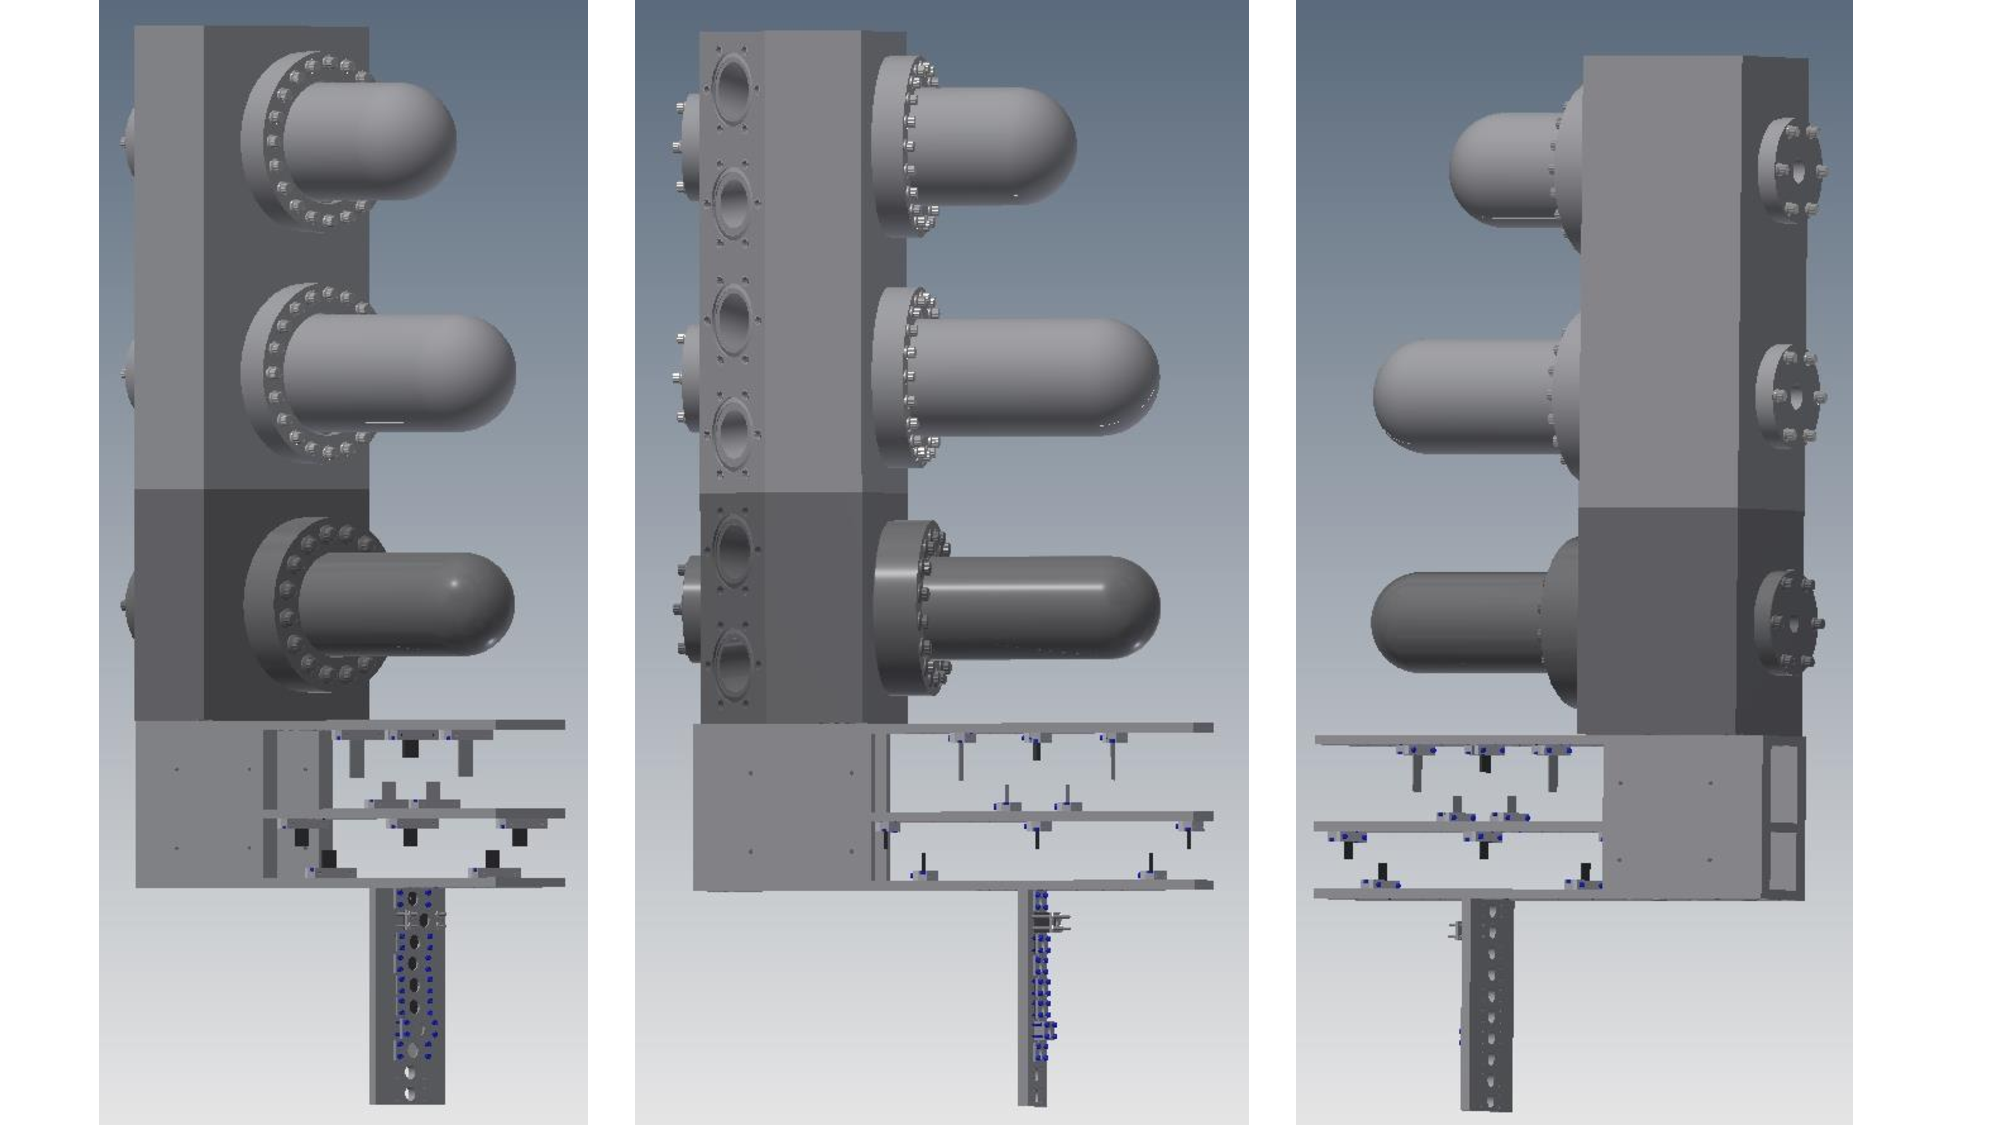
\includegraphics[width =1.0\textwidth]{LoopCAD.pdf}
\end{center}
%\vspace*{0.5cm}
\caption[tgt-layout]{ CAD views of the cryogenic and solid target
  ladders. In this example, there are three cyogenic loops, with one
  cell per loop. The cryo targets are assembled above the solid target
  ladder. Beam enters from the left in the leftmost picture, and from
  the right in the rightmost picture. The middle picture shows the
  hydrogen inlet and outlet manifolds.}
\label{fig:LoopCAD}
\end{figure}
}

A wealth of information about the Hall C cryotarget system is
available at \url{https://userweb.jlab.org/\~smithg/target/Qweak/}.
At that location links to the target training talk can be found, as
well as contact numbers for the target experts, a guide to the control
system (GUIs), a FAQ, descriptions of the essential responsibilities
and how-tos for the target, the operational restrictions (current and
raster limits) for each target, the slow controls archiver, and much
more.
	

\infolevone{
During normal operation, the hydrogen and/or deuterium targets shall
have already been liquefied by the target group and are in a stable
state of about 3 degrees sub-cooled liquid (19.0 K for hydrogen and
22.0 K for deuterium) at pressures of $\sim$24 psia.  The normal
operating conditions of the targets are given in
Table~\ref{tab:target-cryo-param}.  Also listed in
Table~\ref{tab:target-cryo-param} are the freezing and boiling
temperatures. These parameters should be reasonably stable
(temperature to $\pm 0.1$ K, pressure to $\pm 2$ psi) provided that
the End Station Refrigerator (ESR) is stable. The temperature is
controlled by a software PID (Proportional-Integral-Differential
feedback) loop with a high power heater (up to 1500 Watts).  The PID
loop reads the output of one of the temperature sensors and adjusts
the power in the high power heater to keep the temperature
constant. The control loop functions extremely well and the
temperature fluctuations with steady beam are typically measured in
hundredths of degrees. The PID control loop also monitors the electron
beam current to keep the target temperature stable by compensating for
this heat load during unstable beam situations.

\begin{table}
\centering
\begin{tabular}{|c|c|c|c|c|}
\hline 
  & Temperature  & Pressure  & Freezing T & Boiling T \tabularnewline
Target & (\ensuremath{^{\circ}K}) &  (PSIA) &  (\ensuremath{^{\circ}K}) & (\ensuremath{^{\circ}K})
\tabularnewline
\hline 
H\ensuremath{_{2}}
 & 19 $\pm$ 0.1 & 24 $\pm$ 2  & 13.86 & 22.24\tabularnewline
\hline 
D\ensuremath{_{2}}
 & 22 $\pm$ 0.1 & 24 $\pm$ 2 & 18.73 & 25.13\tabularnewline
\hline 
\end{tabular}
\caption[Cryo-target: operation conditions]{Normal operating conditions of the cryo-target cells.}


\label{tab:target-cryo-param} 
\end{table}
}


\infolevone{ 


\section*{Graphical User Interface}

The principal interface with the target is through the Graphical User
Interface (GUI) of the control system. Every target operator must be
familiar with the use of the primary and secondary target GUIs. A
screenshot of the main target GUI is shown in
Fig.~\ref{fig:MainGUI}. In this example, hydrogen is condensed in Loop
3. The status (current values)of the temperatures and pressures
associated with the target loops as well as the coolant is
displayed. In addition the target heater power, recirculation fan
frequency, and JT (coolant) valve opening are procided, along with
information about the selected target and the lifter.

\begin{figure}[!htb]
%\vspace*{-1.8cm}
\begin{center}
%\hspace*{-3.5cm}
%\includegraphics[width =0.95\textwidth,angle=-90]{Pics/QWEAK-tgt-schematic.pdf}
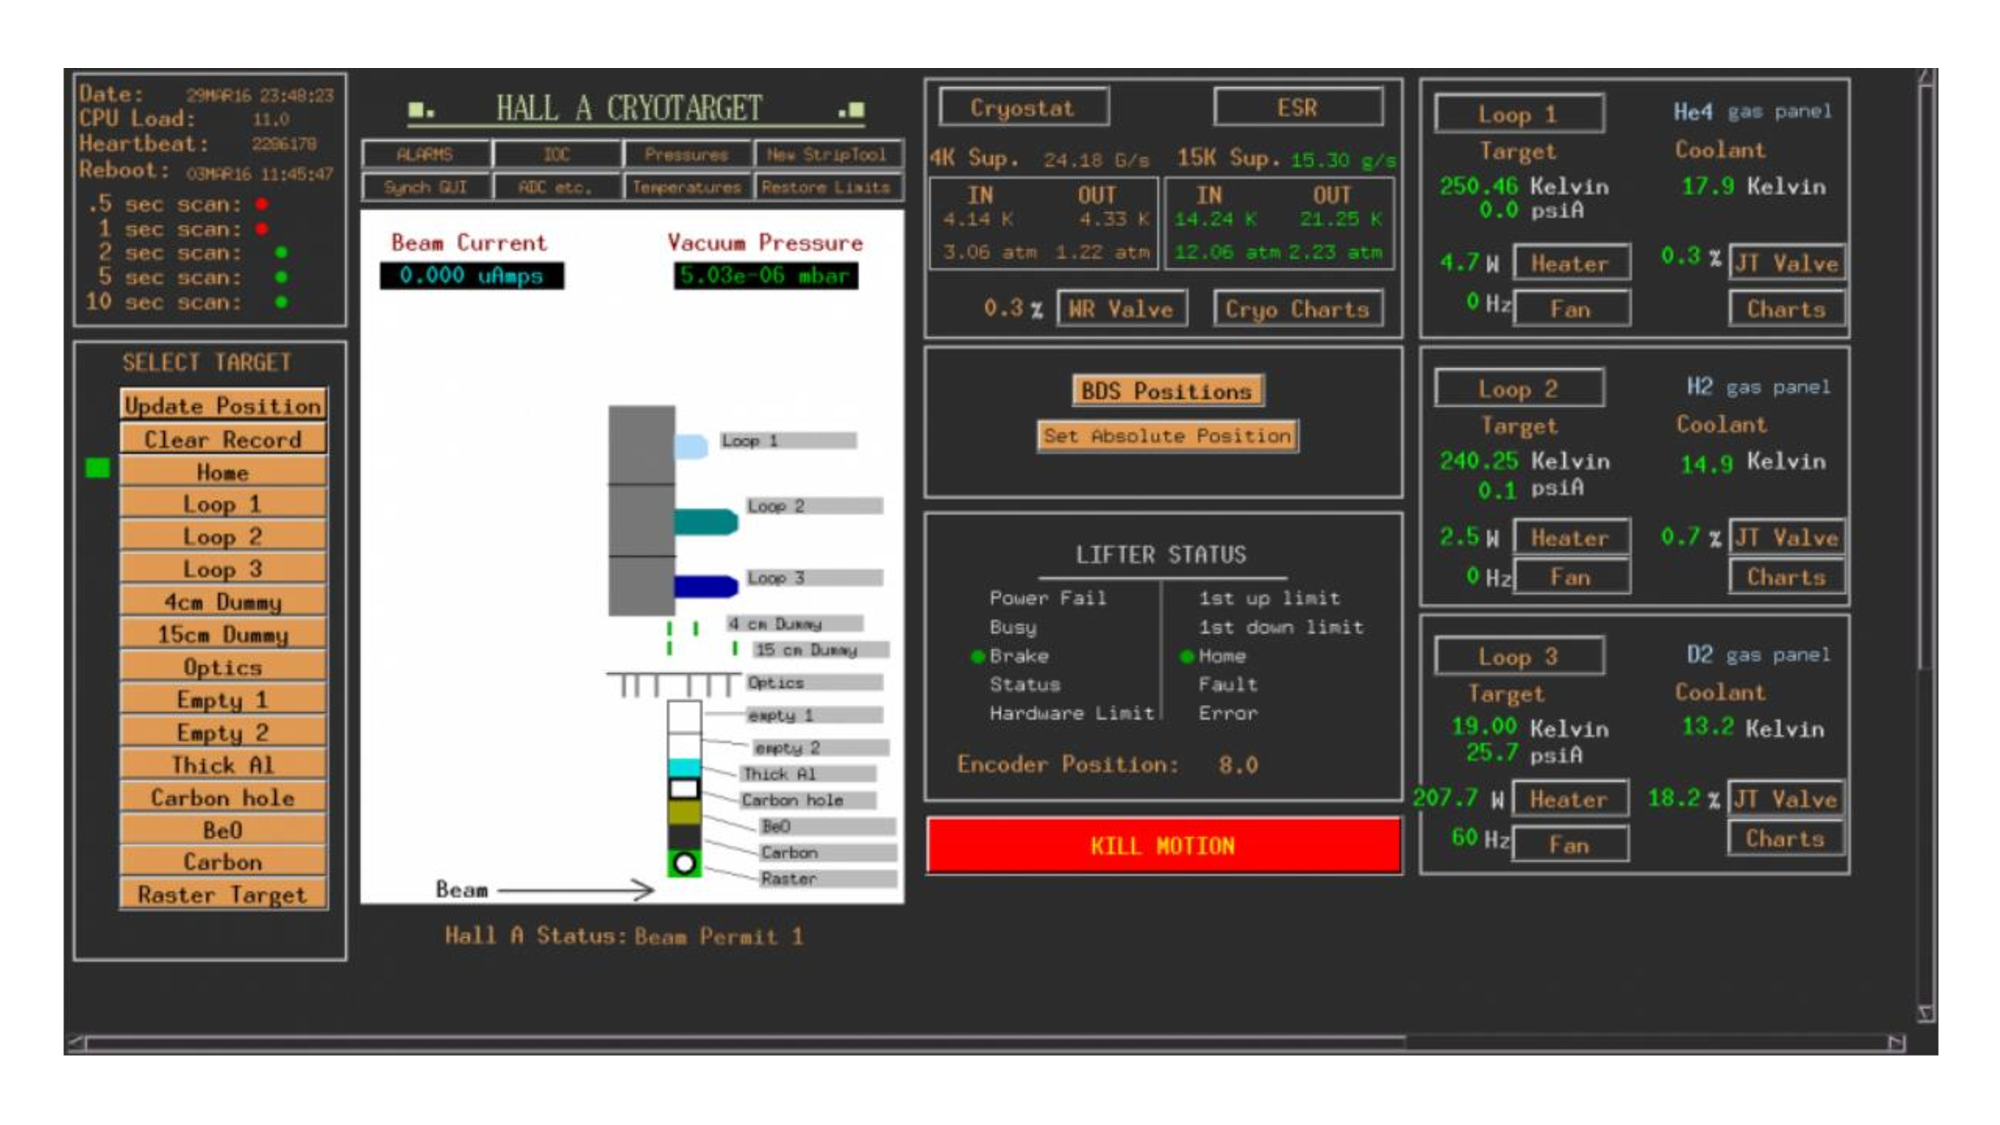
\includegraphics[width =1.0\textwidth]{MainGUI.pdf}
\end{center}
%\vspace*{0.5cm}
\caption[tgt-layout]{ Screenshot of the main target GUI. Loop 3
  contains LH2, the other loops are unused. Secondary GUIs can be
  launched from the buttons on this main GUI. The values of various
  temperature and pressure parameters are green when they are inside
  the alarm limits, and change color when they fall outside the limits
  defined in the alarm handler. }
\label{fig:MainGUI}
\end{figure}


\subsection{Alarm Handler}
}

\begin{safetyen}{0}{0} 
It is \emph{mandatory} to have an audible alarm handler, ALH, running
at all times when the target gas has been condensed.  Further, it is
\emph{mandatory} that the alarm handler be visible in all work spaces
on the target control computer and ``on top'' of other GUIs. It is
further mandatory that all alarms be ``serviced'' in the sense that
each alarm must be investigated. No alarm may ever be ignored.
%\end{safetyen}
While engineered controls ensure personnel and equipment safety, the
alarm handler can save the experimenter lots of time, grief and
potentially prevent problems with data. The ALH will alarm if any of
its parameters go out of normal range. Servicing the alarm is the
responsibility of the target operator. At high beam currents, the ALH
may alarm when the beam goes from on to off or from off to on, if the
high power heater does not respond quickly enough to the change in the
beam heat load, or if there is insufficient reserve heater power
available. The ALH can also repeatedly alarm if there are noisy analog
channels.
%\begin{safetyen}{0}{0}
If the AH alarms repeatedly or the
cause of the alarm is not clear, the target operator should contact
the on-call target expert.
\end{safetyen}
\infolevone{
The ALH GUI and its secondary GUIs are
shown in Fig.~\ref{fig:ALHGui}.

\begin{figure}[!htb]
%\vspace*{-1.8cm}
\begin{center}
%\hspace*{-3.5cm}
%\includegraphics[width =0.95\textwidth,angle=-90]{Pics/QWEAK-tgt-schematic.pdf}
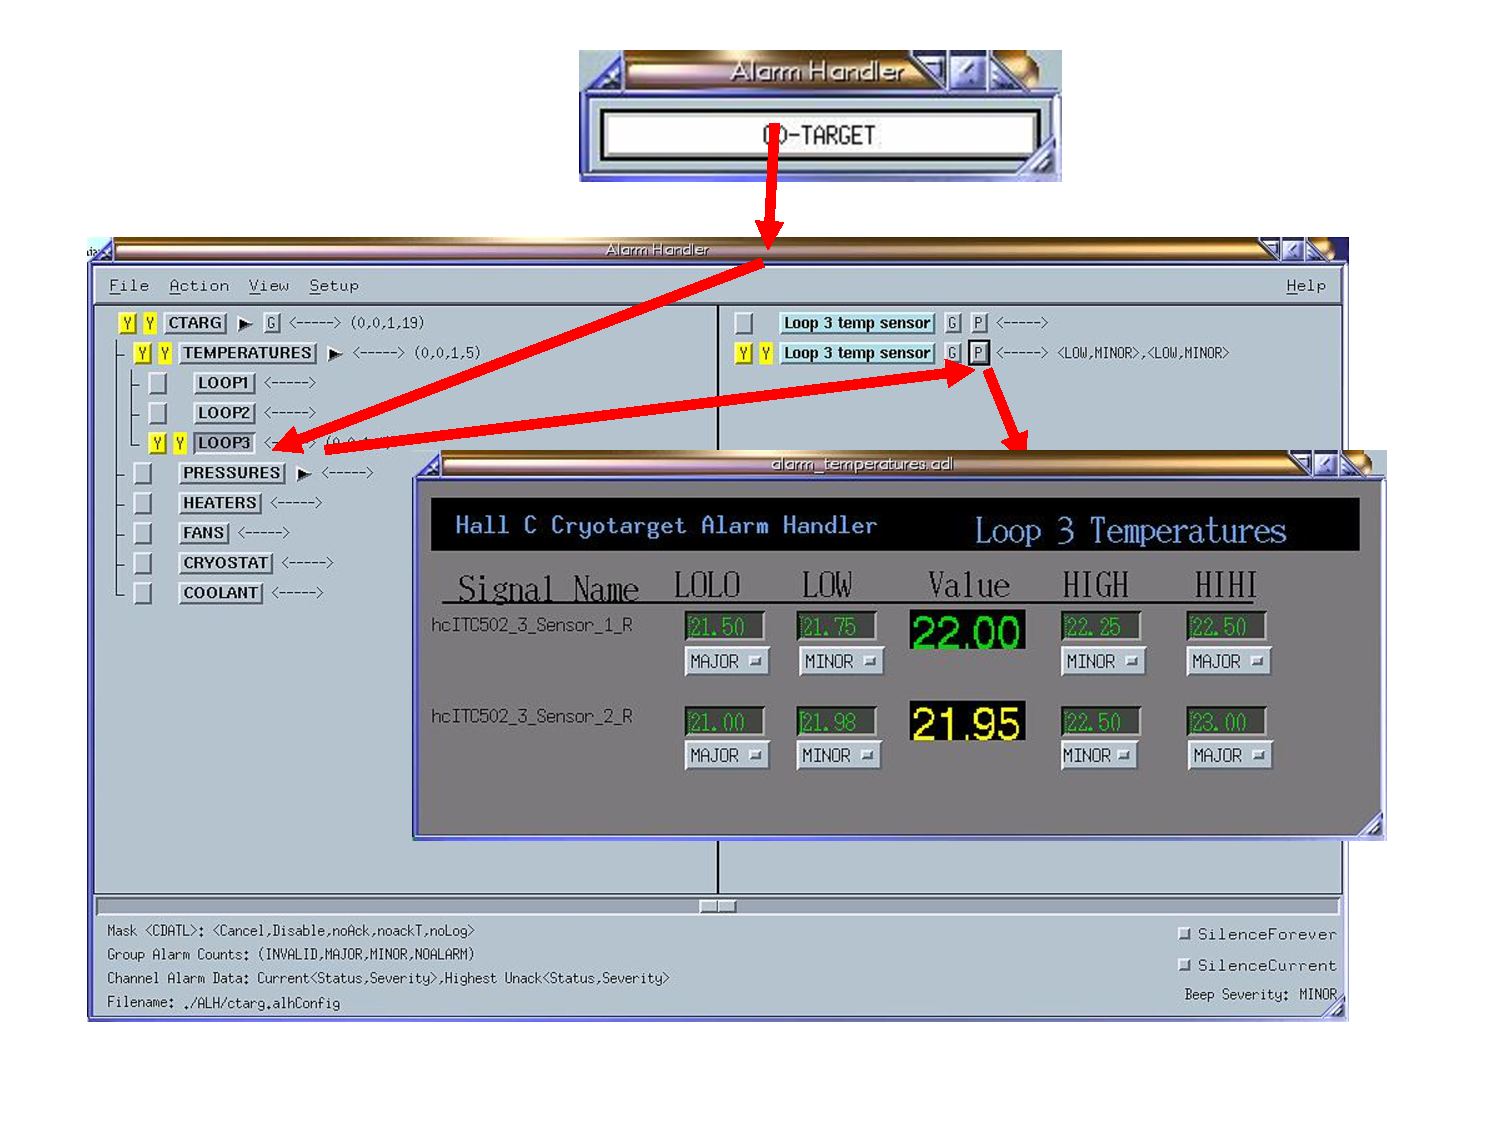
\includegraphics[width =1.0\textwidth]{ALH.pdf}
\end{center}
\vspace*{-1.cm}
\caption[tgt-layout]{ Screenshot of the ALH GUIs. In an alarm state,
  this GUI blinks and beeps. The arrows indicate the steps to service
  the alarm. Pressing the upper GUI brings up the large secondary
  GUI. Pressing the highlighted ``LOOP3'' button on the left brings up
  the LOOP3 branches of the alarm tree on the right. Pressing the
  ``P'' button there brings up a third GUI with the current values and
  alarm limits associated with that particular branch. }
\label{fig:ALHGui}
\end{figure}

}
\infolevone{
\subsection{Target Motion and Fast Raster}

Target motion is interlocked with the machine Fast Shut Down (FSD)
system. Therefore, it is \emph{mandatory} that operators call MCC so
that they can remove beam from the Hall and mask our target-motion FSD
node \emph{before} moving the target. During target motion, the target
operator must watch the target GUI carefully to insure the motion is
going as expected. In case it is not, target motion crash switches are
provided on the GUI and in the counting room.  When target motion has
completed, the MCC must be called again to restore beam and remove
(unmask) the target motion FSD. The target operator must insure that
the requested beam current and raster size are consistent with the
operational restrictions
(\url{http://opweb.acc.jlab.org/internal/ops/ops_webpage/restrictions/ops_restrictions.html})
for the new target. MCC should also perform this check, but the target
operator is the first line of defense. Finally, the target operator
must also insure that adjustments to the cooling power are made, if
necessary, in response to the new target and/or beam current.

\begin{safetyen}{0}{0} 
The intrinsic diameter of the electron beam is typically only 100
$\mu$m. When beam of such a small size hits the cryotarget, there is a
danger that it can melt the aluminum target cell, and/or significantly
reduce the density of the cryogenic target along the path of the beam
through the cell. The former is catastrophic. The latter has a
negative impact on most experiments, but can be characterized with
sufficient precision for many experiments by making additional
measurements as a function of beam current.

The fast raster is used to mitigate these effects by dithering the
beam at the face of the target. At regular intervals, and every time
the target is moved to a new position, the target operator \emph{must
  check to make sure that the fast raster is on} and that it has a
size consistent with that specified in the operational restrictions
for that target. It's best to check the raster setpoints as well as
the raster magnet current readback. In addition, a scope in the
counting room provides an image of the raster pattern as a quick
visual check. Because the raster magnet current is a function of the
beam momentum and desired raster size, it's difficult to set alarm
limits on. As a result we rely on the target operator to check that
the raster is on and working as desired. Unlike the situation found in
Hall A, in Hall C there are no quadrupoles between the raster magnets
and the target. As a result there is a much more robust relationship
between the raster magnet currents and the rastered beam size at the
target.
\end{safetyen}
}


\infolevone{


\subsection{Cryogenic Consumption}

The ESR is not a bottomless reservoir of helium coolant. Typically not
more than 25 g/s of 15 K coolant can be delivered from the ESR, which
must be split between Halls A \& C.  Every effort should be made to
keep our consumption within reasonable bounds. This means that heater
overheads should be tens and not hundreds of Watts and that loops
which will be dormant for extended periods should be powered down as
much as possible.  If the target operator thinks that the cryogenic
consumption is too high (or has received complaints from another ESR
user) and is uncertain about the appropriate action, he/she should
contact the on-call target expert first.

Typical values for the temperature and pressure associated with the
``15 K'' helium coolant supply when running a LH2 target are 14 K and
12 atm. Typical return values are 20 or 21 K, and 2.2 atm. The mass
flow of the coolant is typically 15 g/s, but varies depending on the
beam current and target thickness. The condition of the insulating
vacuum in the transfer lines also impacts the mass flow needed to cool
the target. Unusually large mass flow and/or supply temperature may
indicate that this vacuum space must be pumped out again. A minimum
mass flow of 6 or 7 g/s is needed to keep the transfer lines cold.
}

\infolevone{
\subsection{Checklist}

The Hall C target experts and the JLab target group tracks the state
of the target. To facilitate this task
%the target checklist \emph{must be logged and 
the charts and the main target page screen must be
captured to the HCLog at least once per shift.
%} Do we really need this to be performed? The epics dataloger is more useful for monitoring the system.
}

\infolevone{
\subsection{Target Operators}

One individual on each shift is responsible for target operations
whenever liquid hydrogen or liquid deuterium has been condensed, even
if the experiment is in a ``standby'' mode.  This individual is the
dedicated target operator (TO) and shall have the appropriate training
to keep the target safe and ready to use in the experiment.

Personnel with no previous training must complete the following three
steps to be certified as a TO:
\begin{enumerate}
\item The first step is the ``theoretical part'', which consists of a
  target expert going through the target training talk with you. This
  talk explains the basics, including GUI operation, as well as
  recommended responses to off-normal events. Ideally the prospective
  TO has arranged for this with a target expert well in advance so
  that the talk may be given to a group, instead of individually on a
  case-by-case basis.
\item The second part is a practical, also given by a target expert,
  which usually takes place in the Hall C counting house and consists
  of a hands-on walk through of the control system and some of the
  procedures for handling off normal events. This practical requires
  that the target be condensed. It also should be arranged with a
  target expert in advance so that it can be coordinated with other
  prospective TOs.
\item Finally, the last step requires the new TO to shadow a trained
  TO for (typically) half a shift in order to get more comfortable
  with normal operation. This last step can be accomplished while on
  shift as a shift leader or 3rd, or just by coming to the counting
  room at a convenient time.
\end{enumerate}  

All TOs have to renew their training for the 12 GeV era, because of
the long hiatus in operation during 12 GeV construction. Training
taken for Hall A (12 GeV training) is good for Hall C, and vice
versa. If a TO was already trained for the 6 GeV era but wants to
renew their training for the 12 GeV era, the requirements are simpler.
\begin{enumerate}
\item It is recommended but not required that the training talk be
  attended. In lieu of attending this talk, the training slides can be
  reviewed online at
  \url{https://userweb.jlab.org/~smithg/target/Qweak/HallACTgt_Training.pdf}.
\item A brief practical training is required with a cold target, in
  the counting room, with a target expert, in order to refresh the
  skills of the TO.
\end{enumerate}

After the target operator's training has been completed, he/she should
email one of the target experts so that the TOs name can be added to
the list of trained target operators maintained by the experts.

%The target operator must read this document, the Safety Assessment
%Document for the Hall C Cryogenic Targets, and the short version of
%the GUI manual. 
All of the documentation that must be read and signed by any person on
shift (the COO, RSAD, ESAD, RWP, and any other documents required of
regular shift-takes) must also be read and signed by target operators.
Radiation worker I training must be current, and the TO must have a
valid TLD (radiation dosimeter) in case a target-related entry to the
hall must be made. The target operator shall be familiar with the GUI
system and be able to handle the normal target loop operation, the
cryostat operation and the target motion. He/she shall also be able to
deal with GUI crashes, IOC crashes and the usual alarms.

%if he/she feels comfortable
%with the normal operation of the cryotargets, he/she should sign his/her
%name on the target operator authorization list, which is  maintained in the
%counting house by the target controls, indicating that he/she
%has read this procedure and has been trained. The target expert who
%trained him/her should inform the Hall C staff who is responsible
%for the cryotarget system (G. Smith). 

\begin{safetyen}{0}{0} 

The following table contains the names of the currently recognized
target experts (who have worked on the Hall C cryotarget system and
have extensive knowledge of the system) and their pager numbers.


\begin{table}[h]
\centering
\begin{tabular}{| l | l | l | }
\hline
Group & Name & Contact info    \\ \hline
Hall C & Silviu Covrig & tgt pager: (757) 584-5411 \\ \hline 
Hall A & JianPing Chen & cell: 218-0722 \\ \hline
Cryo-Target Group & Dave Meekins & cell: 968-9076 \\ \hline 
Cryo-Target Group& Christopher Keith & cell: 746-9277 \\ \hline
\end{tabular}
\caption{Cryotarget experts and authorized personnel, with their phone numbers.}
\label{tab:cryotarg:personnel-con}
\end{table}

One cryotarget expert will be on-call 24/7 whenever hydrogen or
deuterium has been condensed.
%is in cooled state. 
The currently on-call target expert will be identified on the white board in the counting house. A list of other cryotarget-experts will be posted
in the Hall C Counting House as well, in case the expert on call cannot be reached.
\end{safetyen}
}

\begin{safetyen}{0}{0} 

\infolevone{
\section{Safety Assessment}

\label{sec:target-cryo-safety}
The Hall C target safety assessment document resides on the target
group's web page at
\url{https://polweb.jlab.org/hallc/Cryotarget/Target\%20Safety\%20Assessment\%20Document1.5.doc}.
  This is the document which contains the safety analyses, detailed
  calculations, and mitigations of the hazards identified for the
  cryotarget. It dates from Feb. 25, 2004. More recent and applicable
  information e.g. calculations, design and fabrication documents,
  testing documentation, etc. are stored in the pressure system
  database and are beyond the scope of this document.

Cryotarget installation, maintenance, and repair is performed
exclusively by the JLab target group (not by users).  The task hazard
analysis worksheet covering such work in the scattering chamber is
\url{https://polweb.jlab.org/hallc/Cryotarget/In\%20chamber\%20work.doc}, and
  that for disconnecting the target is found here:
  \url{https://polweb.jlab.org/hallc/Cryotarget/Disconnect\%20Target.doc}.  A
    guide and checklist used by the target group and occasionally the
    target experts which describes the procedures for determining what
    state the target is in, pumping and purging operations, and warmup
    and cooldown of the targets is at
    \url{https://polweb.jlab.org/hallc/Cryotarget/Target-operation-manual.pdf}.

Target operation is the responsibility of the system owner but, for
practical purposes is the domain of the staff and users on a given
experiment. The users' guide to general operation of the Hall C
cryotarget, prepared by the target group but somewhat dated (March,
2003), is available at
\url{https://polweb.jlab.org/guides/ctarg/CTARG_MAN.html}. The resource
\url{https://userweb.jlab.org/~smithg/target/Qweak/} is a more recent
guide (Feb., 2014) for the general user.
% DGM update this with more correct information from C Keith. Is there a Hall C wiki?
}

\subsection{Hazards}

The cryogenic hydrogen and deuterium targets present a number of
potential hazards, such as fire/explosion hazard of the flammable gas
as well as the hazards connected with the vacuum vessel and cryogenic
liquids (ODH and high pressure). The target system benefits from many
years of experience using it at Jefferson Lab. Hazards, mitigation
measures, and causes and corrective measures associated with past
failures are described in the ``Hydrogen Target Safety Assessment
Document'' at
\url{https://polweb.jlab.org/hallc/Cryotarget/Target%20Safety%20Assessment%20Document1.5.doc}.
\subsection{Mitigations}

\paragraph{Flammable Gas}
\label{sec:targ-flammablegas}

\infolevone{
Hydrogen and deuterium are colorless, odorless gases and hence not
easily detected by human senses. Hydrogen air mixtures are flammable
over a large range of relative concentrations from 4$\%$ to 75$\%$
H$_{2}$ by volume. Detonation can occur with very low energy input,
less than 10\% of that required by mixtures of air and gasoline. At
temperatures above 23 K hydrogen gas is lighter than (STP) air and
hence will rise. At atmospheric pressure, the ignition temperature
is approximately 811 K but air-H$_{2}$ mixtures at pressures of 0.2
to 0.5 Atm can be ignited at temperatures as low as 610 K. Hydrogen
mixtures burn with a colorless flame \cite{bi:mc75}.

The total volume of hydrogen in the target is approximately 7 $l$.
The volume changes between the liquid state and gas at STP by a factor
of about 850. Thus filling the target would require about 6000 STP $l$
of hydrogen. The hydrogen target is connected to a 1,000 Gallon (about
3,800 $l$) recovery tank. The normal running pressure for hydrogen is
about 25 psia. Thus, the total amount of hydrogen in the system is
about 14000 STP $l$. A similar volume of deuterium is required.  In
addition to this volume, two hydrogen bottles (in any combination of
H2 and D2 may be kept in the Hall in order to fill and pump/purge the
targets.  These bottles will be placed in a gas rack behind the gas
panels.  The large storage tanks are located outside the Hall at the
rear of the counting house.
}


The basic idea behind safe handling of any flammable or explosive
gas is to eliminate oxygen (required for burning) and to prevent exposure
to any energy source that could cause ignition. In the Hall C environment,
the most likely source of oxygen is of course the atmosphere and the
most likely ignition sources are from electrical equipment. Oxygen
is removed from the internal volumes of the system by pumping and
purging the system. Extensive procedures reviewed by an independent
expert are used to perform this task. This task shall only be performed
by system experts.

%Hydrogen gas detection shall be installed as part of the Hall C VESDA
%system. This system shall be developed and maintained by Facilities
%Management and Logistics as part of the fire protection system for the
%Hall.

%There are three flammable gas detectors installed (one on top of the
%target, one each on top of the hydrogen and deuterium gas panels)
%to provide early detection of hydrogen/deuterium leaks. These detectors
%are sensitive (and calibrated) over the range from 0 to 50\% Lower
%Explosive Limit (LEL) of hydrogen. The electro-chemical sensors were
%manufactured by Crowcon Detection Instruments LTD and the readout
%(four channels) was purchased from CEA Instruments, Inc. (The Gas
%Master Four System). The readout unit provides two alarm levels per
%channel. The low level alarm is tripped at 20\% of LEL while 40\%
%of LEL activates the high level alarm. Each channel has a relay
%output for both low and high level alarm states and there is also
%a set of common relays for both alarm levels (these common relays
%respond to the logic of the sensor
%inputs). 

%xxx


\infolevone{ 
\paragraph{Electrical Installation}

Hall C contains a significant amount of electrical equipment and
almost all of it could serve as an ignition source in the presence of
an explosive oxygen and hydrogen mixture. Extensive efforts have been
made to minimize the dangers from the equipment that is most likely to
come into contact with hydrogen gas. Electrical equipment considered
to be in close contact with hydrogen meets the requirements of NFPA 2
Hydrogen Technologies Code and/or NFPA 55 Compressed Gases and
Cryogenic Fluids Code as well as NFPA 497. Equipment not meeting these
Code requirements is isolated during off-normal events by either valve
isolation (vacuum turbopumps) or by electrical power trip.

A combination of pressure switchs, installed on the scattering
chamber, will trip when the vacuum in the scattering chamber is
greater than 0.1 and 1 Torr (i.e. during a loss of insulating vacuum
event). These switches de-energize the following systems: vacuum gauge
power, fan motor power, and heater power supplies. The switch also
forces pneumatically actuated gate valves to close, isolating the
turbo pumps. A Machine FSD is issued from the cold cathode gauge
controller when the vacuum pressure exceeds 50 micro Torr.

There are a number of electrically powered devices associated with
the target gas handling system. All the pressure transducers in the
system are approved for use in a hydrogen atmosphere. 
% DGM The solenoid valves on the gas panels are explosion-proof and have been disabled.
The readouts for the pressure transducers are mounted in the target
control equipment racks many meters from the gas panels. All the pressure
transducers have 4--20 mA outputs.

In addition to the electrical devices in the gas handling system,
there are a number of devices inside of or mounted on the scattering
chamber.

All the devices which are in the scattering chamber must have their
power delivered to them by wires in vacuum. The insulation of these
wires must be radiation resistant, so Kapton and glass fiber tubing
insulation has been used where applicable.

The following electrical items are in close proximity to or are actually
in the hydrogen system.
\begin{description}
\item [{\bf Axial Circulation Fan}] The fans which circulate the
  hydrogen in the target are AC induction motors and therefore contain
  no brushes and are practically immune to sparking. The three phase
  (480 V) power for these fans is delivered to them by 18 gauge
  stranded copper wire with Kapton insulation. The maximum current
  that the fans draw is 5 $A$ for a maximum power consumption of 200
  $W$ when pumping liquid hydrogen/deuterium. The current and voltage
  drawn by the fans is monitored by the control system.
\item [{\bf Fan Motor Tachometer}] The fans have a tachometer which
  consists of a coil that views the flux change caused by a permanent
  magnet attached to the motor rotor. The tachometer signals are
  carried on 22 gauge stranded wire with Kapton insulation. This is a
  low power signal. The control system monitors the frequency of the
  fans.
\item [{\bf High Power Heater}] There is a high-power heater in the
  pipe of the loop. The maximum power available is 1500 $W$ (150 V, 10
  A).  The current and voltage supplied to this heater are monitored
  by the control system and there is a software power maximum enforced
  on the power setting of this heater. Internal vacuum connections to
  the heaters are made with 18 gauge stranded wire with Kapton
  insulation.
\item [{\bf Resistive temperature sensors}] There are six resistive
  temperature sensors immersed in each target loop. These resistors
  provide temperature measurements of the target fluid. The
  temperature controllers that read them use a current of less than 30
  $\mu$A to excite them ( they are excited with a constant voltage
  which for our resistors is on the order of 30 mV). The resistors are
  connected to the outside world with quad strand 36 gauge phosphor
  bronze wire with Formvar insulation.
\item [{\bf Target Lifter}] An AC servo motor provides the power to
  lift the target ladder. This motor is powered by three phase 90 $V$
  power and is equipped with fail safe brakes (the brakes are
  \textbf{released} by a loss of 24 $V$ DC control voltage) and 50 to
  1 gear reducers.  On power up, there is a delay relay that ensures
  that the motors are always energized before the brakes are
  released. The motor controller is powered by three phase 208 $V$ and
  is located roughly 10 $m$ from the target.
\item [{\bf Vacuum Pumps}] The scattering chamber is evacuated by two
  Leybold 1000 $l/s$ turbo pumps that are backed by a Leybold 65
  \emph{cfm} mechanical pump. The turbo pumps are powered by 120 $V$
  AC power while the backing pump requires three phase 208 $V$ AC
  power. The turbo pumps are isolated during an insulating vacuum
  failure event by the use of automatic gate valves. The motors on the
  backing pumps are induction motors and approved for use in this
  environment. (The JLab fire protection engineer has reviewed this
  issue). An identical mechanical pump is used in the pump and purge
  system of the gas panels.  Both the scattering chamber backing pump
  and the pump and purge system's mechanical pump exhaust to the vent
  line.
\item [{\bf Vacuum Gauges}] The chamber vacuum is monitored by an HP
  cold cathode gauge. This gauge is not rated for hydrogen service and
  is therefore isolated from the scattering chamber vacuum during an
  insulating vacuum loss event by automatic gate valve. This gauge has
  a maximum operating voltage of 4000 $V$ and a maximum current of 133
  $\mu$A.  The pressure at the entrance to the roughing pump is
  measured by a convectron gauge.
\end{description}
}




\paragraph{Gas Handling System}

The most important aspect of hydrogen safety is to minimize the possibility
of explosive mixtures of hydrogen and oxygen occurring. Therefore
the gas handling system has been made of stainless steel components
(wherever possible) and as many junctions as possible have been welded.
Flanged connections are made with metal seals where possible. Reasonable
measures have been implemented to ensure that the system pressure
does not fall near or below atmospheric pressure.

The pressure in the gas handling system is monitored in numerous places.
Most importantly, the absolute pressure of the target is viewed by
two pressure transducers, one on the fill line, PT127 for H$_{2}$
and PT136 for D$_{2}$, and one on the return line, PT131 for H$_{2}$
and PT140 for D$_{2}$. These pressures are also measured by manual
gauges. The fill line gauges are PI126 for H$_{2}$ and PI135 for
D$_{2}$. The return line gauges are designated PI130, H$_{2}$ and
PI139, D$_{2}$. The gas tanks are viewed with both pressure transducers
(PT133 for hydrogen and PT142 for deuterium) and pressure gauges (PI123
for hydrogen and PI112 for deuterium).


\end{safetyen}

If the pressures significantly deviate either from one another or
from the normal operating pressure, the target operator shall call
the target-expert-on-call. When they differ from one another, it often
is due to a failure of one (or more) of the pressure transducers.
If more than one deviates significantly from the normal operating pressure,
it could be due to temperature change or could be a more serious situation
(i.e. a leak in the system).

The target system is considered by JLab to be a pressure system which
must be in compliance with the requirements of ESH\&Q Manual Chapter
6151. This is a legacy system where the original design and
construction was not in full compliance with the applicable ASME
pressure Codes. A JLab Design Authority shall be responsible for all
alterations and repairs to this system which shall meet the
requirements given in Chapter 6151.  All currently used cells and cell
blocks also meet the requirements of ASME B31.3. Overpressure
protection of all piping components is also in full compliance with
ASME B31.3 The large volume storage tanks located outside the Hall
also meet the requirements of the ASME Boiler and Pressure Code
Section VIII Division 1 and bear a valid ASME nameplate. These tanks
are inspected on a regular basis and currently meet the National Board
NB-23 Code requirements. Overpressure protection of these vessels is
in full compliance with the appropriate division and edition of the
ASME BPVC VIII.


\paragraph{Target Cells}

The target cells themselves represent the most likely failure point in
the hydrogen system. The outer wall is made of 0.006 $in$ thick
aluminum. The entrance and exit windows are thinner, but no less than
0.004 $in$. There is typically one 15 $cm$ long cell bolted on to each
cell block. The cell has an outer diameter of (typically) 3
inches. The upstream windows are connected to 0.8 $in$ diameter tubes
with flanges which are also bolted on to the cell block. A vertical
flow diverter plays a role to make the coolant flow in the vertical
direction to help remove the beam heating more effectively. The cell
and cell block are piping components and have been designed,
fabricated, examined, and tested in compliance with ASME B31.3 (2014)
The design pressure of the current cell is 100 psi. Overpressure
protection is in compliance with ASME B31.3 322.6.3 which allows for
an accumulated overpressure of 120\% of the design pressure.


\paragraph{Pressure Relief}

The gas handling and control systems have been designed to prevent
excessive pressure build up in the system in order to protect the
target cells from overpressure and rupture. It has been determined
that the worst case pressure load will arise from an insulating vacuum
loss. The calculation of this load was reviewed by a JLab Design
Authority not associated with the target group. Under normal
conditions, i.e. vacuum loss with unobstructed return path to storage
vessel, the target safely relieves to the storage vessel.
Overpressure protection, in the form of a reclosing ASME relief valve,
for the target loops (including cells) in compliance with ASME B31.3
322.6.3 is provided on both the supply and return of each loop. These
reliefs exhaust to a dedicated hydrogen exhaust system. The estimated
relief load is 350 scfm of hydrogen The capacity of each relief is
1100 scfm for hydrogen.  The hydrogen exhaust line is 2 inch Sch 10s
IPS stainless steel pipe %\textasciitilde{} $\sim$ 150 ft long capped
by an end of line vent. This line is maintained at a positive pressure
of 1.5 psig using the 4 atm He system.  The scattering chamber and
pump/purge vacuum pumps are also exhausted to this line. Thus any
vented target gas is placed in an inert environment until it is
released outside of Hall C.

\infolevone{
The scattering chamber provides secondary containment in the event
of a cell rupture. Therefore, the scattering chamber itself has a
1 psig relief (check valve), VRV01 and a 4 psig rupture disk. Thus,
the scatting chamber internal pressure will not exceed 5 psig. This
relief path is also exhausted to the hydrogen vent line. A series
of valves and controls allow for the safe removal and exhaust of hydrogen
from the scattering chamber should a cell burst.
}

\paragraph{Scattering Chamber Vacuum}

\label{sec:cryo_targ_cmb_falure}

The scattering chamber will be leak checked before service, but the
possibility of vacuum loss cannot be eliminated. A conservative calculation
estimating the relief load on the relief system of each loop has been
performed. This calculation was performed as part of Code and JLab
policy requirements and was reviewed by an independent JLab Design
Authority. This calculation (TGT-CALC-301-010) has been filed in the
Hall C Cryotarget pressure system directory PS-TGT-XX-026. In summary,
this calculation conservatively indicates that the relief path and
safety devices limit the maximum developed pressure in the cell to
less than the 120 psi for all credible overpressure conditions as
required by ASME B31.3 322.6.3.

\infolevone{
\paragraph{Temperature Regulation}

This is really more an issue of target stability than one of safety.
However, a target with a carefully regulated temperature will presumably
not undergo worrisome pressure changes.

Each target contains six quality temperature measurements with
resistive (Cernox) temperature sensors. The temperature regulation is
performed by a software PID control of a high power heater using one
of the quality temperature measurements as input to the loop. This is
a three parameter control loop (Proportional, Integral and
Differential Control or PID).  The PID loop also compensates for the
beam heat load during beam trip and recovery incidents. This latter
functionality is not a true regulation but rather a one-step
replacement of the beam load should the beam disappear for whatever
reason. The beam load is calculated from the target length, the beam
current as read from a current monitor and the target material.


Excursions of the target temperature outside acceptable limits will
cause alarms, and the 
%control system 
target operator to take action. Finally the redundancy of
temperature measurements can be used 
%by the control system 
to pick
up the failure of a sensor or its readout channel. A more complete
discussion of target temperature regulation is available in Reference
\cite{bi:tgts}. 
}
%XXX


\paragraph{Target Freezing}

Solid hydrogen is more dense than the
liquid phase, so freezing does not endanger the mechanical integrity
of a closed system. The chief hazard is that relief routes out of
the system will become clogged with hydrogen ice, making the behavior
of the system during a warm-up unpredictable. For
this reason, the relief route bypasses the heat exchanger and should
not freeze during any credible scenario. 

\infolevone{ 
The coolant flow through the three target heat exchangers
is connected in parallel for the three target loops. The entire target
system will be operated so that it represents a stable heat load
on the ESR. For instance, the ESR will deliver a constant mass flow
of helium cryogen at a constant temperature of about 15 K (but more typically 14~K), and the coolant
will be returned at an approximately constant but higher temperature,
usually about 20 K.
The targets are temperature regulated by IOC heater PID loop.
}

In the unlikely event that the target temperature drops too low, an
alarm will sound and the target operator shall turn down the corresponding
J-T valve(s) or apply auxiliary heater power. Target temperature
can fall after target IOC reboot. After the reboot the high power heater
will be reset to zero before going back to PID control. Although the
time the high power heater is zero is short (for about 1 minute),
the temperature will drop. To prevent this from happening, an auxiliary
heater is used in parallel to the regular heater. During an IOC reboot,
the auxiliary heater supply will replace the main supply to keep the
temperature from dropping unacceptably. Since 2008, the IOC has been
relocated to the entry labyrinth where the radiation exposure has
been minimized. As a result the frequency of IOC reboots has dramatically
decreased.

\paragraph{ODH}
\label{sec:targ:odh}

The total volume of the targets is relatively small, with the entire
scattering chamber containing only 12000 STP $l$ of target gas when
all three targets are full. As the scattering chamber is located in
the middle of Hall C (i.e. not in a confined area) and the total Hall
C  volume is 26,000 m$^{3}$ (40,000 m$^{3}$ for Hall A), the ODH hazard is minimal. In the event that all the H2 was released into the hall, the oxygen content would drop from 21.0\% to 20.99\%.

\infolevone{
\paragraph{Controls}

The target controls have been implemented with the EPICS~\cite{EPICSwww}
control system and with hardware very similar to that employed by
the accelerator. The basic control functions reside on a VME based
single board computer or IOC. The graphical interfaces to the control
system use a PC, and also require a
%the Hall C Hewlett Packard, HP,
computer for control (HAC) to be present as well. Power failures will
result in a loss of computer control. As a result of such a failure
the target heat exchanger may freeze and the remainder of the target
may vent through the relief path. The beam will also be tripped during
such a failure. There is thus, little chance of damage or danger from
the system. When a power failure occurs, the target operator shall call
the target-on-call immediately.

The principal functions that the control system performs are: 
\begin{description}
\item [{Pressure/Temperature Monitoring}] The pressure and temperature
are monitored at various places in the system and alarm states are
generated if a sensor returns a value that is outside defined limits.
\item [{Target Lifter}] The target lifting mechanism is controlled by
the computer. This allows one to place the desired target in the beam.
Limit switches and hard stops are installed to ensure the target cannot
move outside the allowable range.
\end{description}

Although strip charts are running on the target operator's work station, it can be useful to look further back in time when diagnosing potential problems, or simply answering the question ``Is this normal?''. To this end a simple-to-use archiver interface is provided to interrogate and plot target EPICS variables as a function of time at \url{https://hallcweb.jlab.org/targetlog/}. 
}

\infolevone{
\subsection{Checklist}

Checklist for pre-hall-closing: 
\begin{itemize}
\item Target has completed cool-down, at least one loop has liquid hydrogen
with temperature stable at 19K, pressure stable at around 25 psi. 
\item High power heater in PID control for the hydrogen loop. 
\item Loop fan (pump) has been set to non zero value (20-75 Hz) for the
hydrogen loop. 
\item Coolant (ESR) flow and inlet temperature are stable. 
\item All unused loops are filled with over 1 atm gauge of helium gas. 
\item The target vent line is inerted.
\item Scattering chamber vacuum is normal (below $10^{-5}$). 
\item target in ``Empty/HOME'' position for beam tuning. 
\item Alarm handler is on and all alarm limits are set. 
\item No constant alarms caused by abnormal conditions. 
\item Target-on-call name is written on the whiteboard. 
\item Target EPICS variables are being archived.
\end{itemize}
}

\infoleveqnull{
\paragraph{Further Reading}More detailed
information about the mitigations discussed above can can be 
found in the full Hall C operations manual~\cite{HallCosp}.
}

Any work on this system must be covered by an ePAS Permit To Work (PTW)
\subsection{Responsible Personnel}

The principle contacts for the cryogenic targets were listed in table~\ref{tab:cryotarg:personnel-con}.
Every shift must have a trained target operator whenever the cryogenic
targets contain liquid. These operators are trained by one of the
``experts'' listed in the table and certified by J.P.~Chen or Silviu Covrig. If the target operator suspects issues with the ESR are impacting the target, the target expert on call should be called first. The target expert may then recommend that the cryo expert on call  be contacted through the MCC. 

%\begin{table}[h]
%\centering
%\begin{tabular}{| l | l |}
%\hline
%Beam Parameter & Offset             \\ \hline
%X position & $\pm 125\;\mu$m      \\ \hline
%Y position & $\pm 125\;\mu$m      \\ \hline
%\end{tabular}
%\caption{Typical beam parameter offset during beam modulation}
%\label{tab1}
%\end{table}


\infoleveqnull{
\begin{namestab}{tab:cryotarg:personnel-con}{Cryo Target: personnel
and contacts}{Cryo target: authorized personnel and contacts. ``W.B.''
stands for the white board in Counting House.}
\namestabheader{Hall C Technicians}
\TechonCall{Vacuum}
%\AndyKenyon{Vacuum}
\namestabheader{Hall A/C Physicists}
\CryotargonCall{Cryotarget}
\SilviuCovrig{Cryotarget}
\JianPingChen{Cryotarget}
\namestabheader{JLab Cryo-Target Group}
\DaveMeekins{}
\ChristopherKeith{}
\namestabheader{Central Helium Liquefier (CHL) Experts}
\CryoonCall{ESR}
\CHLgroup{ESR}
\end{namestab}
}



